\documentclass[a4paper, 12pt,]{scrartcl}



\usepackage[utf8]{inputenc}

\usepackage[ngerman]{babel}
\usepackage{amssymb}
\usepackage[T1]{fontenc}
\usepackage{mathtools}
\usepackage{amsmath}
\usepackage{ntheorem}
\usepackage{bbm}
\usepackage{dsfont}
\usepackage{color}
\usepackage{slashed}
\usepackage{hyperref}
\usepackage{graphicx} 
\usepackage{bm}
\usepackage{mathabx}
\usepackage{float}
\usepackage{mwe}
\usepackage{multirow}
\begin{document}
\begin{titlepage}
	\centering
	{\scshape\LARGE Universität Tübingen \par}
	\vspace{2cm}
	{\huge\bfseries Sterling Motor \par}
	\vspace{2cm}
	{\Large \scshape Blockpraktikum 2021} \par
	\vspace{2cm}
	{\Large  Erste Version} \par
	\vspace{2cm}
	{\Large\itshape \underline{Christian Gommeringer} \space \space  \underline{Matthias Gatter}\par}
	\vfill 
	{\large betreut von Jan Riedelsheimer}
	\vfill

	{\large \today\par}
\end{titlepage}
\newpage 
%\tableofcontents 

%\newpage
%\section{Einleitung}
%\begin{flushleft}



%\end{flushleft}
% > < | 
\section{Theorie}
Unseren Überlegungen zugrunde liegt der Sterling Kreisprozess
\begin{figure}[H]\centering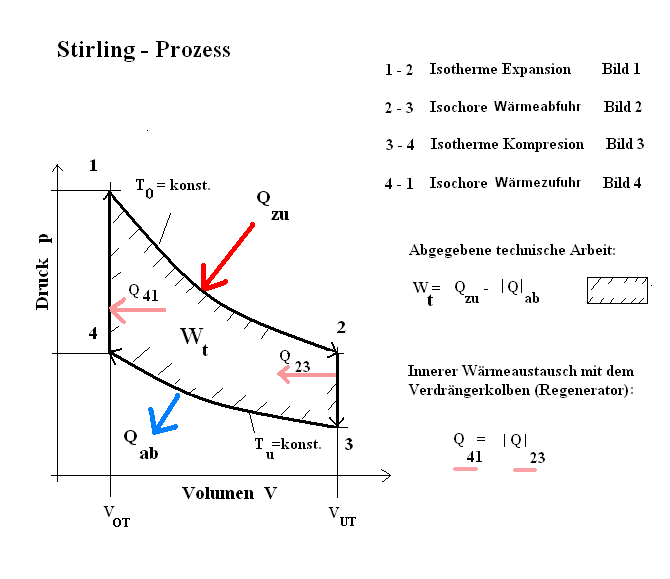
\includegraphics[scale=0.5]{Stirling-Prozess_3}\caption{Abbildung des stirlingschen Kreisprozesses aus Wikipedia}\end{figure}
Wenn wir ihn in der oben abgebildeten Reihenfolge durchlaufen, lässt sich die Wärme, die vom Arbeitsgas mit den Wärmebädern ausgetauscht wurde, in folgende Abschnitte aufteilen
\begin{gather*}\Delta{Q}_{12}=\text{ln}\left(\frac{V_2}{V_1}\right)\,n\,R\,T_1\\
\Delta{Q}_{23}=C_v\,(T_3-T_1)\\
\Delta{Q_{34}}=-\text{ln}\left(\frac{V_2}{V_1}\right)\,n\,R\,T_3\\
\Delta{Q_{41}}=C_v\,(T_1-T_3)\end{gather*}
Hierbei ist $T_1>T_3$. Dies wollen wir in den gesamten folgenden Überlegungen beibehalten. Betrachten wir nun die Energieaustauschbilanz der Wärmebäder, erhalten wir diese indem wir den Energieaustauschs des Arbeitsgases negieren. Damit lässt sich die Bilanz $\Delta{Q_{B_1}}$ für das wärmere Bad mit Temperatur $T_1$ und für das kältere Bad $\Delta{Q_{B_2}}$ aufstellen.
\begin{gather*}\Delta{Q_{B_1}}=-\Delta{Q}_{12}-\Delta{Q_{41}}=-\text{ln}\left(\frac{V_2}{V_1}\right)\,n\,R\,T_1-C_v\,(T_1-T_3)\\
\Delta{Q_{B_2}}=-\Delta{Q}_{34}-\Delta{Q_{23}}=\text{ln}\left(\frac{V_2}{V_1}\right)\,n\,R\,T_3+C_v\,(T_1-T_3)\end{gather*}
Die Beschreibung bezog sich jetzt zuerst auf die Bilanzen beim Betrieb als Wärme-Kraft-Maschine. Der gleiche Wärmetransport wird auch geleistet wenn das System durch einen externen Motor in dieser Richtung betrieben wird (im folgenden wird dieser Umlaufsinn als Umlaufsinn1 bezeichnet). Hier wird Wärmebad 1 gekühlt und Wärmebad 2 beheizt. Der Vorteil des Betriebs durch den Motor, ist dass sich so durch mehr Umdrehungen pro Minute eine stärkere Kühlleistung erbringen lässt oder überhaupt eine Kühlleistung, falls der Temperatur zu gering ist um die Wärmekraftmaschine überhaupt in Gang zu bringen. Die Kühlwirkung bezieht sich auf das Wärmebad 1, das in unserem Fall der Zylinderkopf ist. \newline
Durch Umkehren des Durchlaufs des Stirling Prozesses lässt sich der Zylinderkopf auch heizen. Hier ist allerdings zu beachten, dass von $1\rightarrow4$ das kältere Wärmebad Wärme aufnimmt und von $3\rightarrow2$ das Wärmebad 1 Wärme abgibt. Die Bilanz für die Wärmebäder ergibt sich daher als
\begin{gather*}\Delta{Q_{B_1}}'=\text{ln}\left(\frac{V_2}{V_1}\right)\,n\,R\,T_1-C_v\,(T_1-T_3)\\
\Delta{Q_{B_2}}'=C_v\,(T_1-T_2)-\text{ln}\left(\frac{V_2}{V_1}\right)\,n\,R\,T_3\end{gather*}
Diese Betriebsrichtung fand in unserem Versuch allerdings keine Anwendung.
Die thermodynamisch genutzte Arbeit lässt sich damit durch $\Delta{Q_{B_1}}$ und $\Delta{Q_{B_2}}$ darstellen, und ist der Vollständig halber für beide Umlaufrichtungen hier angegeben.

\begin{align*}W_{pV}=&\Delta{Q}_{12}+\Delta{Q_{34}}\\
=&-(\Delta{Q_{B_1}}+\Delta{Q_{B_2}})\\
W_{pV}'=&-\Delta{Q}_{12}-\Delta{Q_{34}}\\
=&\Delta{Q_{B_1}}'+\Delta{Q_{B_2}}'\end{align*}
Wenn wir nun ein reales System betrachten, findet immer auch Reibung statt. Mit der Annahme, dass beide Wärmebäder die gleiche Reibungswärme zugeführt bekommen, sind $\Delta{Q_{B_1}}$ und $\Delta{Q_{B_2}}$ auf folgende Weise umzuschreiben.
\begin{align*}\Delta{Q_{B_1}}=&-\text{ln}\left(\frac{V_2}{V_1}\right)\,n\,R\,T_1-C_v\,(T_1-T_3)+\Delta{Q_R}\\
\Delta{Q_{B_2}}=&\text{ln}\left(\frac{V_2}{V_1}\right)\,n\,R\,T_3+C_v\,(T_1-T_3)+\Delta{Q_R}\end{align*}
Für die thermodynamisch genutzte Arbeit bedeutet das
\begin{align*}W_{pV}&=-(\Delta{Q_{B_1}}-\Delta{Q_R}+\Delta{Q_{B_2}}-\Delta{Q_R})\\
=&-(\Delta{Q_{B_1}}+\Delta{Q_{B_2}})+2\,\Delta{Q_R}\end{align*}
Wir können daraus zudem die mechanische Arbeit des Motors berechnen, die sich aus der thermodynamisch genutzten Arbeit und der verlorengegangenen Wärme zusammensetzt.
\begin{align*}W_\text{Mech}=&W_{pV}+2\,\Delta{Q_R}\\=&-(\Delta{Q_{B_1}}+\Delta{Q_{B_2}})+4\,\Delta{Q_R}\end{align*}
An dieser Stelle möchte ich noch erwähnen, dass für den zweiten Umlaufsinn, die Reibungswärme, die sich im ersten Fall bei der Berechnung der mechanischen Arbeit der Motors aufsummiert, jetzt gerade aufhebt. Es gilt ohne Reibung
\begin{align*}W_\text{Mech}=\Delta{Q_{B_1}}+\Delta{Q_{B_2}}\end{align*}
und mit Reibung
\begin{align*}W_\text{Mech}=&\Delta{Q_{B_1}}-\Delta{Q_R}+\Delta{Q_{B_2}}\Delta{Q_R}+2\,\Delta{Q_R}\\
=&\Delta{Q_{B_1}}+\Delta{Q_{B_2}}\end{align*}

\section{Versuchsdurchführung}
Wir führten unser Experiment mit einem Stirling Motor der Firma LD Didaktik durch, der mit einem Arbeits- und Verdrängungskolben arbeitet.
\begin{figure}[H]\centering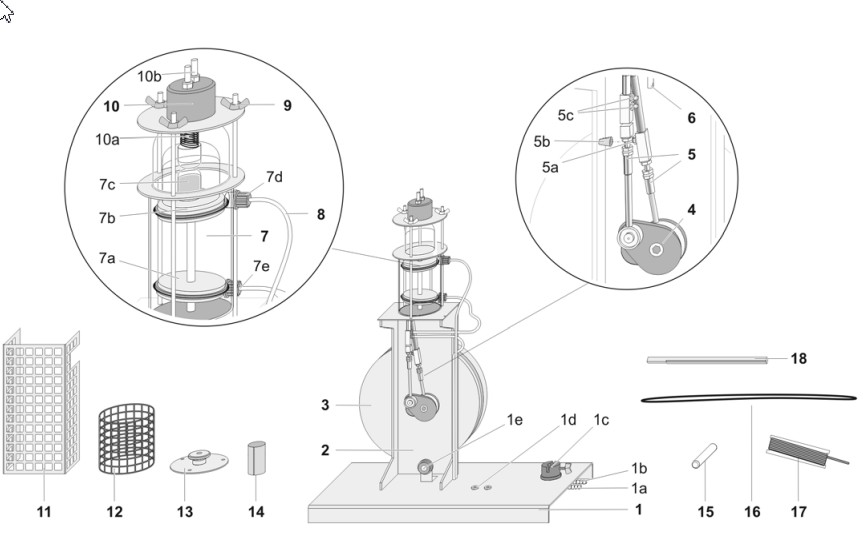
\includegraphics[scale=0.8]{Stirlingmotor}\caption{Aufbau des Stirlingmotors; 7a ist z.B. der Arbeitskolben und 7b der Verdrängungskolben;7d Kühlwasserabfluss;7e Kühlwasserzufluss;10a Heizspirale}\end{figure}

Wir betrieben den Stirlingmotor im Umlaufsinn 1. Als Wärmebäder benutzen wir zum Einen das Kühlwasser, was unser Wärmebad 2 darstellt, und das mit einer gewissen Geschwindigkeit $\text{d}m/\text{d}t$ durch das System gepumpt wurde, und zum Anderen eine Heizspirale im Zylinderkopf als Wärmebad 1. Dies ist so zu verstehen, dass wir hier durch die Heizwendel mit einer bestimmten elektrischen Leistung geheizt hatten, und abwarteten, bis sich die Temperatur im Zylinderkopf auf einen Gleichgewichtswert eingestellt hatte. In diesem Zustand können wir davon ausgehen das in guter Näherung die gesamte elektrische Leistung, in den thermodynamischen Prozess einfließt. Somit beträgt die vom Wärmebad 1 abgegebene Arbeit $\Delta{Q_{B_1}}=-P_{el}\cdot{\tau}$, wobei $\tau$ die Zeit eines Durchlaufs des Stirlingprozesses ist.
Die Wärme die das Wärmebad 2, also das Wasser aufnahm, bestimmten wir dadurch, dass wir die Temperatur $T_1$ des Kühlwassers unmittelbar nach Druchlauf durch den Stirlingmotor maßen. Aus der Differenz zur Temperatur des Kühltanks konnte die ans Wasser abgegebene Wärme berechnet werden.
\begin{equation*}\Delta{Q_{B_2}}=c_{V,\text{Wasser}}\,\Delta{T}\,\frac{\text{d}m}{\text{d}t}\,\tau\end{equation*}

Vor der eigentlichen Messung bestimmten wir noch die Reibungswärme $\Delta{Q_R}$, indem wir den Stirlingmotor bei geöffneten Zylinder betrieben. Dadurch traten keine Volumen und Druckänderungen auf und es fand kein thermodynamischer Prozess statt. Die Wärme, die dabei an das Wasser abgegeben wurde, entsprach hier $\Delta{Q_R}$.

Beim eigentlichen Versuch gingen wir dann wie oben beschrieben vor. Für 5 verschiedene Heizströme, warteten wir bis die Gleichgewichtstemperatur, die zwischen 10°C und 50°C lag, erreicht wurde, und maßen die Temperatur des Kühlwassers $T_1$.

Als zweiter Versuch betrieben wir den Stirlingmotor ohne externen Motor als Wärme-Kraft-Maschine. Dazu heizten wir den Motor über die Heizwendel im Zylinderkopf. Hierbei zeichnete ein Laser der auf ein Spiegelsystem im Stirlingmotor gerichtet war ein maßstabsgetreues p-V Diagramm an die Wand, das wir abzeichneten.

\section{Auswertung}
Wir betrieben den Stirlingmotor mit einer Frequenz von 1 Hz. Als erste Messung bestimmten wir die Durchflussmenge des Kühlwassers 5 mal.
\begin{table}[H]\centering\begin{tabular}{cc}gestoppte Zeit in s&gemessener Wasserdurchfluss in kg\\30&0.11\\60&0.19\\60&0.19\\120&0.36\\60&0.185\end{tabular}\caption{gemessener Wasserdurchfluss in Abhängigkeit der Zeitdauer}\end{table}

Daraus berechnet sich der Durchflussstrom zu 
$$\frac{\text{d}m}{\text{d}t}=3.22\,\frac{g}{s}$$
Die Temperatur des Wassertanks betrug 24.1°C und die Temperatur des Kühlwasser nach Durchlauf war im Leerlaufbetrieb $T_1=25.2°C$. Damit berechnet sich die Reibungswärme zu 
\begin{equation*}\Delta{Q_R}=0.00296\,J\end{equation*}
Wir benutzten hierfür eine spezifische Wärmekapazität für Wasser von $C_{V,\text{Wasser}}=4.84\,J/(kg\,K)$ (Wikipedia).\newline\newline
Als nächstes maßen wir die Wärmemengen $\Delta{Q_{B_1}}$ und $\Delta{Q_{B_2}}$ für verschiedene Gleichgewichtstemperaturen $T_\text{zyl}$ im Zylinderkopf. Beziehungsweise wir maßen $T_1$, Heizstrom $I_H$, Heizspannung $U_H$ der Heizwendel, sowie die elektrische Leistung des externen Motors $P_M$.
\begin{table}[H]\centering\begin{tabular}{c|ccccc}
$T_\text{zyl}$ in °C&10&17.5&27&41.5&55\\\hline
$T_1$ in °C&28	&28.2	&28.4	&28.8	&29.3\\
$I_H$ in A&1.46	&1.57	&1.75	&1.93	&2.16\\
$U_H$ in V&13	&14	&15.4	&17	&19\\
$P_M$ in W&89	&87.6	&87.3	&85.4	&83.4\end{tabular}
\caption{Messung zur Bestimmung von $\Delta{Q_{B_1}}$ und $\Delta{Q_{B_2}}$ für verschieden Gleichgewichtstemperaturen. Die Temperatur des Kühlwassertanks $T_0$ ist unverändert 24.1°C}\end{table}
Daraus lassen sich die Wärmemengen berechnen.
\begin{table}[H]\centering\begin{tabular}{c|ccccc}
$T_\text{zyl}$ in °C&10&17.5&27&41.5&55\\\hline
$\Delta{Q_{B_1}}$ in J&3.7966&4.396&5.39&6.562&8.208\\
$\Delta{Q_{B_2}}$ in J&0.0105&0.0110&0.0116&0.0126&0.014\end{tabular}
\caption{berechnete Wärmemengen}\end{table}
Hieraus lassen sich nach 
\begin{align*}W_{pV}=-(\Delta{Q_{B_1}}+\Delta{Q_{B_2}})+2\,\Delta{Q_R}\end{align*}
wiederum die jeweilige thermodynamisch genutzte Arbeit bestimmen
\begin{table}[H]\centering\begin{tabular}{c|ccccc}
$T_\text{zyl}$ in °C&10&17.5&27&41.5&55\\\hline
$W_{pV}$ in J&3.79143&4.39089&5.38435&6.55528&8.19993\end{tabular}
\caption{thermodynamisch genutzte Arbeit}\end{table}
Die effektive äußere Kennzahl der Wärme Pumpe
\begin{equation*}\varepsilon_{A}=\frac{P_{el}\,\tau}{P_M\,\tau}\end{equation*}
sowie die innere Kennzahl
\begin{equation*}\varepsilon_{I}=\frac{P_{el}\,\tau}{W_{pV}}\end{equation*}
und den mechanischen Wirkungsgrad des externen Motors
\begin{align*}\eta=\frac{W_\text{Mech}}{P_M\,\tau}\\
=&\frac{-(-P_{el}\,\tau+\Delta{Q_{B_2}})+4\,\Delta{Q_R}}{P_M\,\tau}\end{align*}
sind in folgender Tabelle zusammengefasst
\begin{table}[H]\centering\begin{tabular}{c|ccccc}
$T_\text{zyl}$ in °C&10&17.5&27&41.5&55\\\hline
$\varepsilon_A$&0.21326	&0.25091	&0.30871	&0.38419	&0.49209\\
$\varepsilon_I$&1.00121	&1.00116	&1.00105	&1.00103	&1.00098\\
$\eta$&0.21333	&0.25096	&0.30872	&0.38414	&0.49196\end{tabular}
\caption{Leistungszahlen und Wirkungsgrad des Motors für die verschiedenen Temperaturen.}\end{table}

Bestimmen wir nun die Kennzahlen für das Wärmebad 2 (Wasser), betrachten wir den Aspekt der Wärmepumpe. Die äußere Kennzahl soll analog berechnet werden
\begin{equation*}\varepsilon_{A,W}=\frac{\Delta{Q_{B_2}}}{P_M\,\tau}\end{equation*}
Bei der Bestimmung der inneren Leistungszahl soll noch die Reibungswärme von$\Delta{Q_{B_2}}$ abgezogen werden.
\begin{equation*}\varepsilon_{I,W}=\frac{\Delta{Q_{B_2}}-\Delta{Q_R}}{P_M\,\tau}\end{equation*}
\begin{table}[H]\centering\begin{tabular}{c|ccccc}
$T_\text{zyl}$ in °C&10&17.5&27&41.5&55\\\hline
$\varepsilon_{A,W}$&0.00059	&0.00063	&0.00066	&0.00074	&0.00084\\
$\varepsilon_{I,W}$&0.00199	&0.00184	&0.0016	&0.00148	&0.00134\end{tabular}
\caption{äußere und innere Leistungszahl für die Wärmepumpe}\end{table}







Für den Wirkungsgrad der Wärmepumpe ergibt sich beispielsweise
\begin{equation*}\eta_M=\frac{\text{ln}\left(\frac{V_2}{V_1}\right)\,n\,R\,T_1-C_v\,(T_1-T_3)}{\text{ln}\left(\frac{V_2}{V_1}\right)\,n\,R\,(T_1-T_3)+Q_R}\end{equation*}
oder in aus der Messung zugänglichen Größen
\begin{gather*}\eta_M=\frac{W_M-\Delta{Q_{B_2}}'-\Delta{Q_R}}{W_M}\\
\eta_M=\frac{W_M+\Delta{Q_{B_2}}-\Delta{Q_R}}{W_M}\end{gather*}











$\Delta{Q_R}$ wird beim ``Leerlauf'' des Systems aus der erzeugten Wärme berechnet. Sie bezieht sich auf einen Zyklus des Durchlaufs, die mit der Frequenz $f$ aufeinander folgen. 
\begin{equation}\Delta{Q_R}=C_{c,\text{Wasser}}\,(\tilde{T}-T_0)\,\frac{\text{d}m}{\text{d}t}\,\frac{1}{f}\end{equation}
$\tilde{T}$ wird an einem Thermometer an der Austrittsstelle des Kühlwassers aus dem System abgelesen und misst die Temperatur der Wassermenge ($\text{d}m/\text{d}t\,1/f$) die gerade den Kühlprozess abgeschlossen hat. $T_0$ ist die Temperatur im Wasserreservior, aus der das Kühlwasser entnommen wird. Diese Herangehensweise kann aufgrund obiger Überlegungen nur Näherungswerte liefern, da es quasi keinen ``Leerlauf'' gibt, dieser so jedenfalls nicht erreicht wird, sondern die Wärme-/ Kältepumpe auch hier arbeitet. Da die beiden Wärmebäder allerdings die gleiche Temperatur haben, kann man vielleicht argumentieren, dass dieser Effekt gering ist.











\section{Fragen}
Ich habe das, was du für uns auf die Tafel geschrieben hast noch. Ich weiß aber nicht mehr, was die Symbole heißen.  Außerdem würde ich gerne nochmal die Begriffe aus Aufgabe 2 mit dir abklären, weil ich bei deren Bedeutung nicht sicher bin. Das sind also die Fragen:
\begin{itemize}
\item[a)]Wofür steht der Index H in deinen Bezeichnungen?

\item[b)]Ist $P_M$ die mechanische Leistung des Motors oder die elektrische? Dann wäre $W_{pV}$ wahrscheinlich die ``thermodynamisch genutzte Energie'' und es würde gelten $W_{pV}=W_M-Q_R$ (wenn $P_M$ die mechanische Leistung ist). Stimmt das? (wenn nicht, was ist dann $W_{pV}$?)

\item[c)]Sind $I_H$ und $U_H$ die Stromstärke und Spannung, mit denen der Motor betrieben wurde. Dann wäre der Wirkungsgrad des Motors $\eta_\text{Motor}=P_M/(I_H\,U_H)$?

\item[d)]Sehr wichtig ist noch, ob ich die Identifikation richtig habe: ``transportierte Wärme'' ist $\Delta{Q_{B_1}}$ für die ``Kältemaschine'' und ``abgegebene Wärme'' ist $\Delta{Q_{B_1}}'$ für die ``Wärmepumpe''.

\item[e)]Wir haben nur $T_H$ gemessen, so haben wir es jedenfalls bezeichnet. Aber ich glaube $T_H$ ist die Temperatur des Kühlwassers nach Durchlauf. $T_K$ haben wir nicht gemessen. Ist das ein Problem? $T_\text{zyl}$ haben wir allerdings schon gemessen.

\item[f)]Was ist dein $Q_\text{ges}$
 \end{itemize}








\end{document}